\subsection{Fairness methods}
After defining fairness in a mathematical sense, the question arises how a classifier can be modified to satisfy the chosen definition of fairness. This is what fairness methods deal with.
Depending on their position in the machine learning pipeline, we distinguish between:
\begin{enumerate}
    \item Pre-processing methods
    \item In-processing methods
    \item Post-processing methods
\end{enumerate}
Pre-processing methods follow the idea that the data should be modified before training, so that the algorithm learns on "corrected" data. Reweighing observations before training is an example for a preprocessing method. The idea is to assign different weights to the observations based on relative frequencies, so that the algorithm learns on a balanced dataset (\cite{caton2024}).\\
In-Processing methods modify the optimization criterion, such that it also accounts for a chosen fairness metric. Introducing a regularization term to the loss function is one example of such modifications.\\
Post-processing methods work with black box algorithms, just like preprocessing methods. We only need the predictions from the model to adjust them so that again a chosen fairness metric is fulfilled. One example for this is thresholding, where we set group specific thresholds to re-classify the data after training (\cite{hardt2016}).
Depending on the task (regression, classification) and the model there are highly specified and advanced methods. For the case study in chapter 3, we limit ourselves to methods implemented in the \texttt{mlr3fairness} package.
% mlr3fairness currently has two preprocessing methods, one postprocessing method and several fairness adjusted models implemented. We decide to use a reweighing methods that works with assigning weights to the observations to equalise the distribution of $P(Y|PA)$.
% The inprocessing method is a fairness-adjusted logistic regression implemented in mlr3fairness inspired by Zafar et. al. This method optimises for statistical parity (independence). The postprocessing method we choose aims for equalised odds and it works by randomly flipping a subset of predictions with pre-computed probabilities in order to satisfy equalised odds constraints.

\subsection{Bias and the feedback loop}
Before applying the theory to real-world data, it remains to introduce different types of biases and the context in which a machine learning model is usually embedded.
Deployed as an ADM, the model assists in decisions such as whether someone gets admitted to college, receives a loan or is released from prison. It thereby indirectly contributes to shaping our reality.\\
\cite{mehrabi2022} conceptualise the situation in form of the \textit{data, algorithm, and user interaction feedback loop} (\autoref{fig:bias_loop}), which can be understood as follows.
We as a society make decisions, which are reflected in our reality. The reality is made measurable by collecting data. The algorithm learns from this data to make an optimal prediction, on which the decision-maker bases their judgement. The new choice will shape our reality again, which reflects in updated data.\\ 
At each stage, bias can be introduced into the process. More dangerous, bias can even be amplified as the algorithm influences decision-making on a large scale.
Consequently, every fairness project comes with the responsibility to understand the data-generating process and gain clarity on how the algorithm will be deployed in the real world.\\
Moreover, the \textit{data, algorithm, and user interaction feedback loop} helps clarify which type of bias might be relevant in a given situation by placing it at a specific position in the feedback loop. Distinguishing between bias mechanisms can be crucial and should influence the definition of fairness and the choice of fairness adjustments in a given situation. This will also become evident in the following section where we examine the SQF dataset.

\begin{figure}
    \centering
    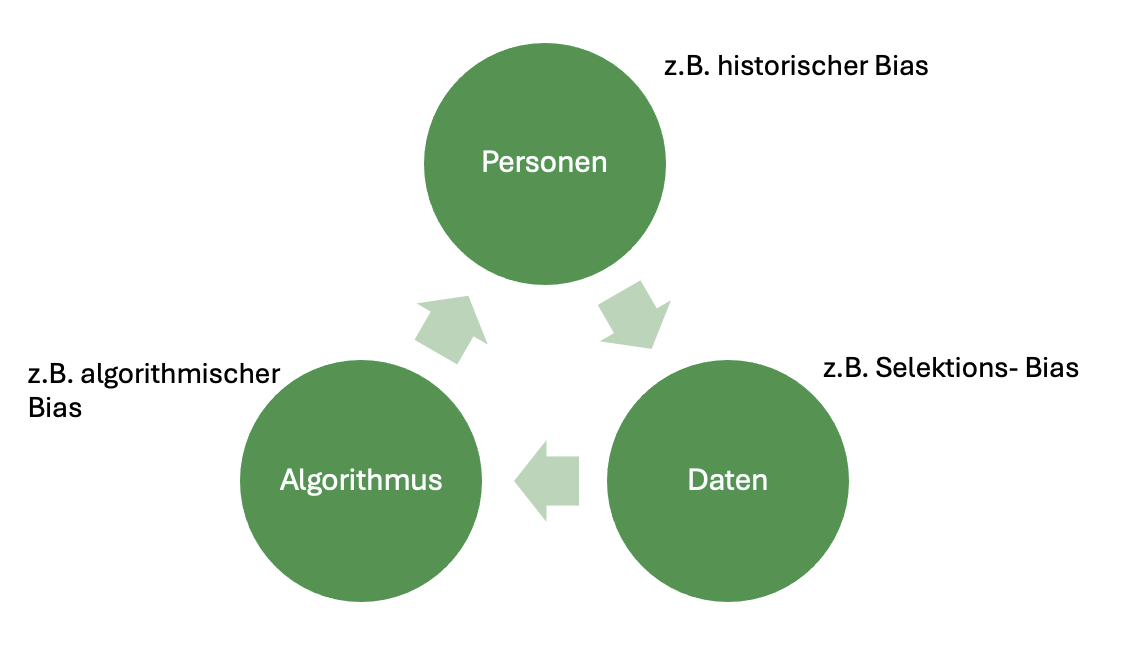
\includegraphics[width=0.7\textwidth]{../figures/bias_loop.png}
    \caption{The \textit{data, algorithm, and user interaction feedback loop} as described by \cite{mehrabi2022}. Different categories of bias can be introduced at each stage of the process.}
    \label{fig:bias_loop}
\end{figure}

% \subsection*{Bias}
% We want to end this general introduction into fair machine learning by outlining the context in which the algorithm is usually embedded. On this note we also advice practitioners to think about the source of bias that could be present in your situation, as this \textit{should} influence how fairness is defined and what fairness adjustments are appropriate. This will motivate the potential difficulties that can arise when implementing fairness in the real world.
% \cite{caton2024} describe the situation as follows. The algorithm is embedded in a feedback loop with the user and data.
% We as a society make decision, which reflect our reality. We make our reality measurable by collecting data. The algorithm learns from this data and makes predictions, on which we base new decisions. 
% At each of these three points bias can be introduced into the process and, above all, bias can also be reinforced in the course of this process.
% In the context of the Stop, Question, and Frisk data, historical bias and selection bias are probably the most relevant sources of bias.
% Historical bias can shows itself in different ways. In our case it would mean that we assume that some people in our data have repeatedly experienced discrimination in terms of being arrested.
% Selection bias refers to the fact that the data is not representative of the population of New York City, because the decision to stop someone is based on a biased decision policy.



